\subsection{Grapple}
Grappling is holding an opponent in hand-to-hand combat, very common in smaller gladiatorial arenas. For monsters, it can mean locking you in its mouth, or holding you down in the ground.

\subsubsection{Grapple Checks}
Repeatedly in a grapple, you need to make opposed grapple checks against an opponent. A grapple check is like a melee attack roll. Your attack bonus on a grapple check is:

{
	\centering
	\vskip1em
	\Large \textit{Base attack bonus} + \textit{Str. modifier}\\ + \textit{special size modifier}
	\vskip1em
}

\textbf{Special Size Modifier:} The special size modifier for a grapple check is as follows: Colossal +16, Gargantuan +12, Huge +8, Large +4, Medium +0, Small $-4$, Tiny $-8$, Diminutive $-12$, Fine $-16$. Use this number in place of the normal size modifier you use when making an attack roll.

\subsubsection{Starting a Grapple}
To start a grapple, you need to grab and hold your target. Starting a grapple requires a successful melee attack roll. If you get multiple attacks, you can attempt to start a grapple multiple times (at successively lower base attack bonuses).

\begin{enumerate*}
\item \textbf{Attack of Opportunity.} You provoke an attack of opportunity from the target you are trying to grapple. If the attack of opportunity deals damage, the grapple attempt fails. (Certain monsters do not provoke attacks of opportunity when they attempt to grapple, nor do characters with the Improved Grapple feat.) If the attack of opportunity misses or fails to deal damage, proceed to Step 2.

\item \textbf{Grab.} You make a melee touch attack to grab the target. If you fail to hit the target, the grapple attempt fails. If you succeed, proceed to Step 3.

\item \textbf{Hold.} Make an opposed grapple check as a free action. If you succeed, you and your target are now grappling, and you deal damage to the target as if with an unarmed strike.

If you lose, you fail to start the grapple. You automatically lose an attempt to hold if the target is two or more size categories larger than you are.

In case of a tie, the combatant with the higher grapple check modifier wins. If this is a tie, roll again to break the tie.

\item \textbf{Maintain Grapple.} To maintain the grapple for later rounds, you must move into the target's space. (This movement is free and doesn't count as part of your movement in the round.) Moving, as normal, provokes attacks of opportunity from threatening opponents, but not from your target.

If you can't move into your target's space, you can't maintain the grapple and must immediately let go of the target. To grapple again, you must begin at Step 1.
\end{enumerate*}

\subsubsection{Grappling Consequences}
While you're grappling, your ability to attack others and defend yourself is limited.

\textbf{No Threatened Squares:} You don't threaten any squares while grappling.

\textbf{No Dexterity Bonus:} You lose your Dexterity bonus to AC (if you have one) against opponents you aren't grappling. (You can still use it against opponents you are grappling.)

\textbf{No Movement:} You can't move normally while grappling. You may, however, make an opposed grapple check to move while grappling.

\subsubsection{If You're Grappling}
When you are grappling (regardless of who started the grapple), you can perform any of the following actions. Some of these actions take the place of an attack (rather than being a standard action or a move action). If your base attack bonus allows you multiple attacks, you can attempt one of these actions in place of each of your attacks, but at successively lower base attack bonuses.

\textbf{Activate a Magic Item:} You can activate a magic item, as long as the item doesn't require spell completion activation. You don't need to make a grapple check to activate the item.

\textbf{Attack Your Opponent:} You can make an attack with an unarmed strike, natural weapon, or light weapon against another character you are grappling. You take a $-4$ penalty on such attacks.

You can't attack with two weapons while grappling, even if both are light weapons.

\textbf{Cast a Spell:} You can attempt to cast a spell while grappling or even while pinned (see below), provided its casting time is no more than 1 standard action, it has no somatic component, and you have in hand any material components or focuses you might need. Any spell that requires precise and careful action is impossible to cast while grappling or being pinned. If the spell is one that you can cast while grappling, you must make a Concentration check (DC 20 + spell level) or lose the spell. You don't have to make a successful grapple check to cast the spell.

\textbf{Damage Your Opponent:} While grappling, you can deal damage to your opponent equivalent to an unarmed strike. Make an opposed grapple check in place of an attack. If you win, you deal nonlethal damage as normal for your unarmed strike (1d3 points for Medium attackers or 1d2 points for Small attackers, plus Strength modifiers). If you want to deal lethal damage, you take a $-4$ penalty on your grapple check.

\textit{Exception:} Monks deal more damage on an unarmed strike than other characters, and the damage is lethal. However, they can choose to deal their damage as nonlethal damage when grappling without taking the usual $-4$ penalty for changing lethal damage to nonlethal damage.

\textbf{Draw a Light Weapon:} You can draw a light weapon as a move action with a successful grapple check.

\textbf{Escape from Grapple:} You can escape a grapple by winning an opposed grapple check in place of making an attack. You can make an Escape Artist check in place of your grapple check if you so desire, but this requires a standard action. If more than one opponent is grappling you, your grapple check result has to beat all their individual check results to escape. (Opponents don't have to try to hold you if they don't want to.) If you escape, you finish the action by moving into any space adjacent to your opponent(s).

\textbf{Move:} You can move half your speed (bringing all others engaged in the grapple with you) by winning an opposed grapple check. This requires a standard action, and you must beat all the other individual check results to move the grapple.

\textit{Note:} You get a +4 bonus on your grapple check to move a pinned opponent, but only if no one else is involved in the grapple.

\textbf{Retrieve a Spell Component:} You can produce a spell component from your pouch while grappling by using a full-round action. Doing so does not require a successful grapple check.

\textbf{Pin Your Opponent:} You can hold your opponent immobile for 1 round by winning an opposed grapple check (made in place of an attack). Once you have an opponent pinned, you have a few options available to you (see below).

\textbf{Break Another's Pin:} If you are grappling an opponent who has another character pinned, you can make an opposed grapple check in place of an attack. If you win, you break the hold that the opponent has over the other character. The character is still grappling, but is no longer pinned.

\textbf{Use Opponent's Weapon:} If your opponent is holding a light weapon, you can use it to attack him. Make an opposed grapple check (in place of an attack). If you win, make an attack roll with the weapon with a $-4$ penalty (doing this doesn't require another action).

You don't gain possession of the weapon by performing this action.

\subsubsection{If You're Pinning an Opponent}
You can attempt to damage your opponent with an opposed grapple check, you can attempt to use your opponent's weapon against him, or you can attempt to move the grapple (all described above). At your option, you can prevent a pinned opponent from speaking.

You can use a disarm action to remove or grab away a well secured object worn by a pinned opponent, but he gets a +4 bonus on his roll to resist your attempt.

You may voluntarily release a pinned character as a free action; if you do so, you are no longer considered to be grappling that character (and vice versa).

You can't draw or use a weapon (against the pinned character or any other character), escape another's grapple, retrieve a spell component, pin another character, or break another's pin while you are pinning an opponent.

\begin{figure*}[t!]
\centering
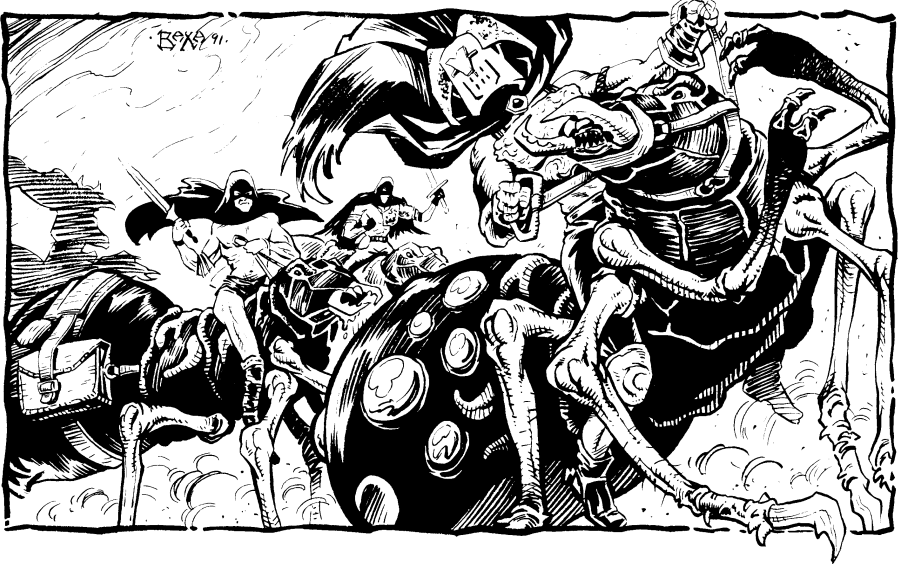
\includegraphics[width=\textwidth]{images/raiders-1.png}
\WOTC
\end{figure*}

\subsubsection{If You're Pinned by an Opponent}
When an opponent has pinned you, you are held immobile (but not helpless) for 1 round. While you're pinned, you take a $-4$ penalty to your AC against opponents other than the one pinning you. At your opponent's option, you may also be unable to speak. On your turn, you can try to escape the pin by making an opposed grapple check in place of an attack. You can make an Escape Artist check in place of your grapple check if you want, but this requires a standard action. If you win, you escape the pin, but you're still grappling.

\subsubsection{Joining a Grapple}
If your target is already grappling someone else, you can use an attack to start a grapple, as above, except that the target doesn't get an attack of opportunity against you, and your grab automatically succeeds. You still have to make a successful opposed grapple check to become part of the grapple.

If there are multiple opponents involved in the grapple, you pick one to make the opposed grapple check against.

\subsubsection{Multiple Grapplers}
Several combatants can be in a single grapple. Up to four combatants can grapple a single opponent in a given round. Creatures that are one or more size categories smaller than you count for half, creatures that are one size category larger than you count double, and creatures two or more size categories larger count quadruple.

When you are grappling with multiple opponents, you choose one opponent to make an opposed check against. The exception is an attempt to escape from the grapple; to successfully escape, your grapple check must beat the check results of each opponent.